\documentclass[1p]{elsarticle_modified}
%\bibliographystyle{elsarticle-num}

%\usepackage[colorlinks]{hyperref}
%\usepackage{abbrmath_seonhwa} %\Abb, \Ascr, \Acal ,\Abf, \Afrak
\usepackage{amsfonts}
\usepackage{amssymb}
\usepackage{amsmath}
\usepackage{amsthm}
\usepackage{scalefnt}
\usepackage{amsbsy}
\usepackage{kotex}
\usepackage{caption}
\usepackage{subfig}
\usepackage{color}
\usepackage{graphicx}
\usepackage{xcolor} %% white, black, red, green, blue, cyan, magenta, yellow
\usepackage{float}
\usepackage{setspace}
\usepackage{hyperref}

\usepackage{tikz}
\usetikzlibrary{arrows}

\usepackage{multirow}
\usepackage{array} % fixed length table
\usepackage{hhline}

%%%%%%%%%%%%%%%%%%%%%
\makeatletter
\renewcommand*\env@matrix[1][\arraystretch]{%
	\edef\arraystretch{#1}%
	\hskip -\arraycolsep
	\let\@ifnextchar\new@ifnextchar
	\array{*\c@MaxMatrixCols c}}
\makeatother %https://tex.stackexchange.com/questions/14071/how-can-i-increase-the-line-spacing-in-a-matrix
%%%%%%%%%%%%%%%

\usepackage[normalem]{ulem}

\newcommand{\msout}[1]{\ifmmode\text{\sout{\ensuremath{#1}}}\else\sout{#1}\fi}
%SOURCE: \msout is \stkout macro in https://tex.stackexchange.com/questions/20609/strikeout-in-math-mode

\newcommand{\cancel}[1]{
	\ifmmode
	{\color{red}\msout{#1}}
	\else
	{\color{red}\sout{#1}}
	\fi
}

\newcommand{\add}[1]{
	{\color{blue}\uwave{#1}}
}

\newcommand{\replace}[2]{
	\ifmmode
	{\color{red}\msout{#1}}{\color{blue}\uwave{#2}}
	\else
	{\color{red}\sout{#1}}{\color{blue}\uwave{#2}}
	\fi
}

\newcommand{\Sol}{\mathcal{S}} %segment
\newcommand{\D}{D} %diagram
\newcommand{\A}{\mathcal{A}} %arc


%%%%%%%%%%%%%%%%%%%%%%%%%%%%%5 test

\def\sl{\operatorname{\textup{SL}}(2,\Cbb)}
\def\psl{\operatorname{\textup{PSL}}(2,\Cbb)}
\def\quan{\mkern 1mu \triangleright \mkern 1mu}

\theoremstyle{definition}
\newtheorem{thm}{Theorem}[section]
\newtheorem{prop}[thm]{Proposition}
\newtheorem{lem}[thm]{Lemma}
\newtheorem{ques}[thm]{Question}
\newtheorem{cor}[thm]{Corollary}
\newtheorem{defn}[thm]{Definition}
\newtheorem{exam}[thm]{Example}
\newtheorem{rmk}[thm]{Remark}
\newtheorem{alg}[thm]{Algorithm}

\newcommand{\I}{\sqrt{-1}}
\begin{document}

%\begin{frontmatter}
%
%\title{Boundary parabolic representations of knots up to 8 crossings}
%
%%% Group authors per affiliation:
%\author{Yunhi Cho} 
%\address{Department of Mathematics, University of Seoul, Seoul, Korea}
%\ead{yhcho@uos.ac.kr}
%
%
%\author{Seonhwa Kim} %\fnref{s_kim}}
%\address{Center for Geometry and Physics, Institute for Basic Science, Pohang, 37673, Korea}
%\ead{ryeona17@ibs.re.kr}
%
%\author{Hyuk Kim}
%\address{Department of Mathematical Sciences, Seoul National University, Seoul 08826, Korea}
%\ead{hyukkim@snu.ac.kr}
%
%\author{Seokbeom Yoon}
%\address{Department of Mathematical Sciences, Seoul National University, Seoul, 08826,  Korea}
%\ead{sbyoon15@snu.ac.kr}
%
%\begin{abstract}
%We find all boundary parabolic representation of knots up to 8 crossings.
%
%\end{abstract}
%\begin{keyword}
%    \MSC[2010] 57M25 
%\end{keyword}
%
%\end{frontmatter}

%\linenumbers
%\tableofcontents
%
\newcommand\colored[1]{\textcolor{white}{\rule[-0.35ex]{0.8em}{1.4ex}}\kern-0.8em\color{red} #1}%
%\newcommand\colored[1]{\textcolor{white}{ #1}\kern-2.17ex	\textcolor{white}{ #1}\kern-1.81ex	\textcolor{white}{ #1}\kern-2.15ex\color{red}#1	}

{\Large $\underline{12a_{0822}~(K12a_{0822})}$}

\setlength{\tabcolsep}{10pt}
\renewcommand{\arraystretch}{1.6}
\vspace{1cm}\begin{tabular}{m{100pt}>{\centering\arraybackslash}m{274pt}}
\multirow{5}{120pt}{
	\centering
	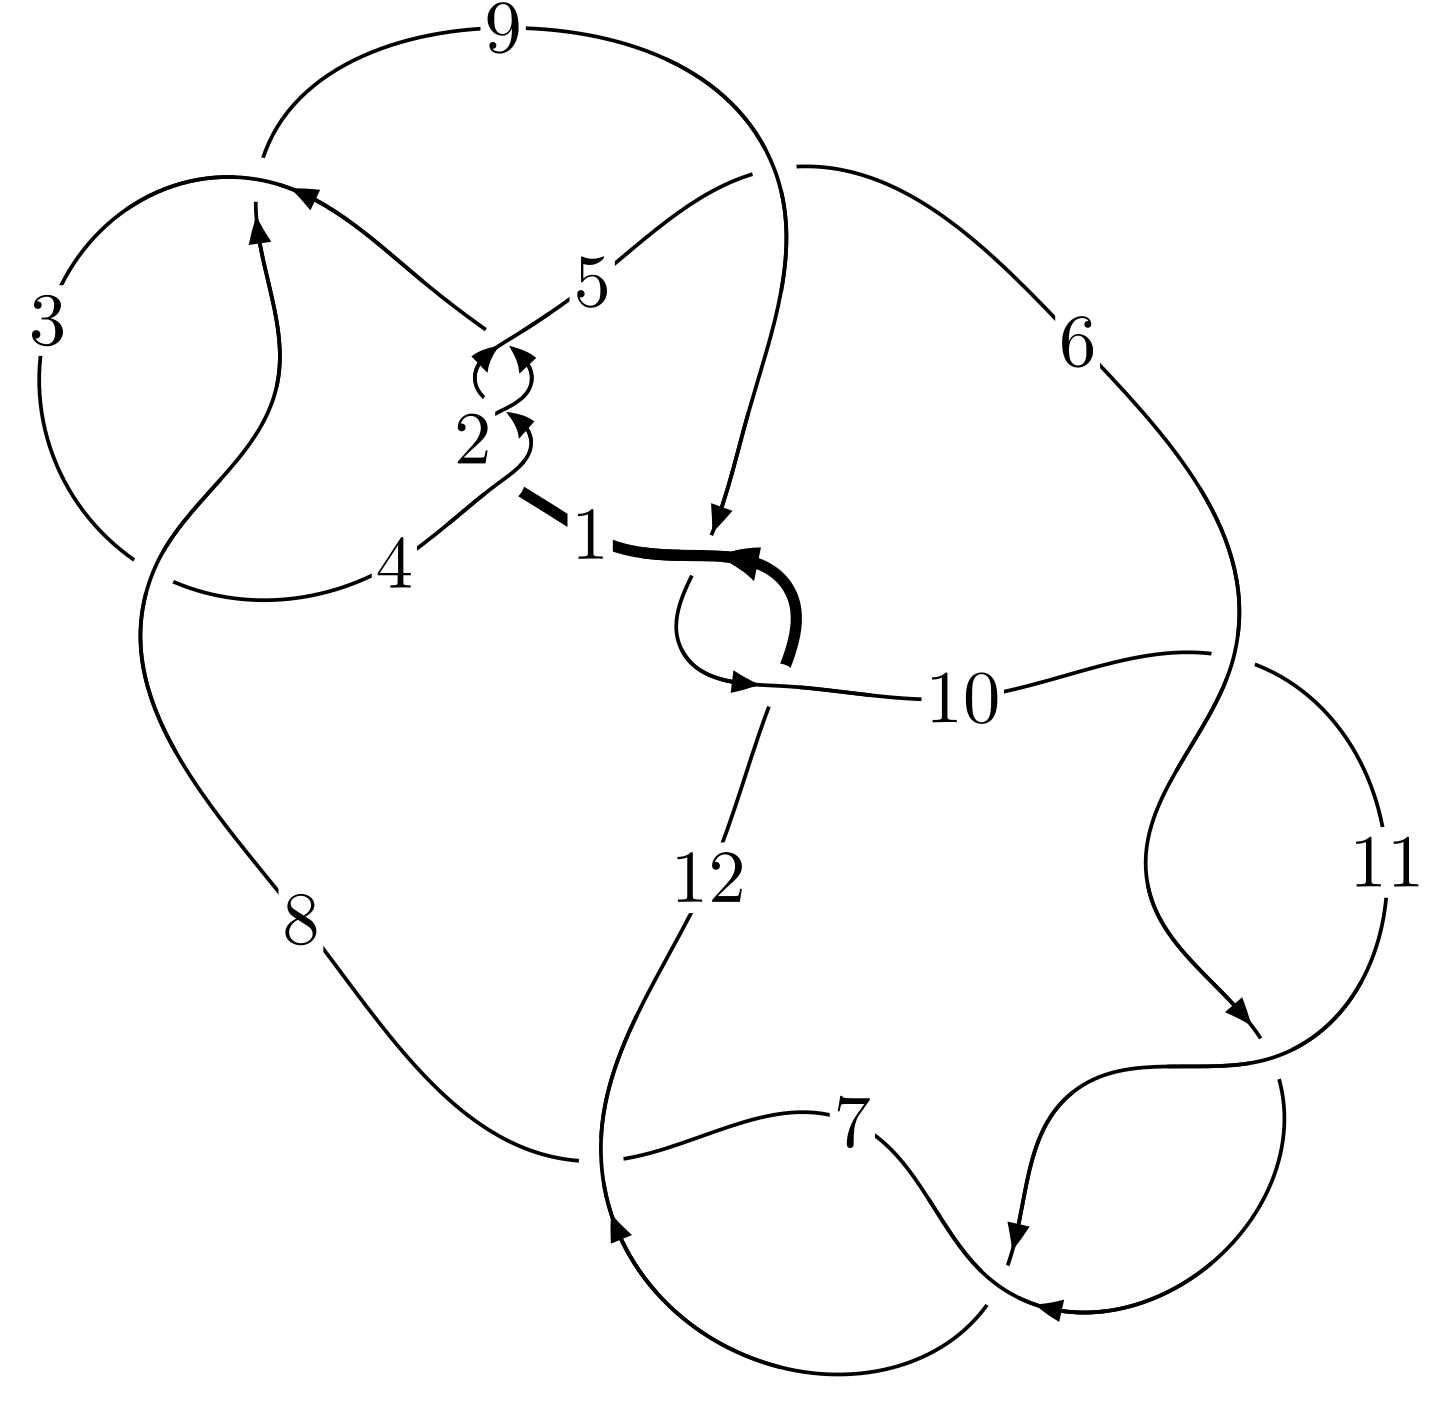
\includegraphics[width=112pt]{../../../GIT/diagram.site/Diagrams/png/1623_12a_0822.png}\\
\ \ \ A knot diagram\footnotemark}&
\allowdisplaybreaks
\textbf{Linearized knot diagam} \\
\cline{2-2}
 &
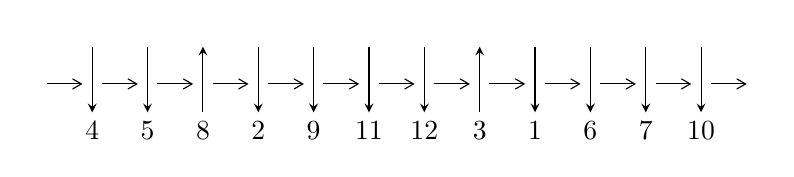
\begin{tikzpicture}[x=20pt, y=17pt]
	% nodes
	\node (C0) at (0, 0) {};
	\node (C1) at (1, 0) {};
	\node (C1U) at (1, +1) {};
	\node (C1D) at (1, -1) {4};

	\node (C2) at (2, 0) {};
	\node (C2U) at (2, +1) {};
	\node (C2D) at (2, -1) {5};

	\node (C3) at (3, 0) {};
	\node (C3U) at (3, +1) {};
	\node (C3D) at (3, -1) {8};

	\node (C4) at (4, 0) {};
	\node (C4U) at (4, +1) {};
	\node (C4D) at (4, -1) {2};

	\node (C5) at (5, 0) {};
	\node (C5U) at (5, +1) {};
	\node (C5D) at (5, -1) {9};

	\node (C6) at (6, 0) {};
	\node (C6U) at (6, +1) {};
	\node (C6D) at (6, -1) {11};

	\node (C7) at (7, 0) {};
	\node (C7U) at (7, +1) {};
	\node (C7D) at (7, -1) {12};

	\node (C8) at (8, 0) {};
	\node (C8U) at (8, +1) {};
	\node (C8D) at (8, -1) {3};

	\node (C9) at (9, 0) {};
	\node (C9U) at (9, +1) {};
	\node (C9D) at (9, -1) {1};

	\node (C10) at (10, 0) {};
	\node (C10U) at (10, +1) {};
	\node (C10D) at (10, -1) {6};

	\node (C11) at (11, 0) {};
	\node (C11U) at (11, +1) {};
	\node (C11D) at (11, -1) {7};

	\node (C12) at (12, 0) {};
	\node (C12U) at (12, +1) {};
	\node (C12D) at (12, -1) {10};
	\node (C13) at (13, 0) {};

	% arrows
	\draw[->,>={angle 60}]
	(C0) edge (C1) (C1) edge (C2) (C2) edge (C3) (C3) edge (C4) (C4) edge (C5) (C5) edge (C6) (C6) edge (C7) (C7) edge (C8) (C8) edge (C9) (C9) edge (C10) (C10) edge (C11) (C11) edge (C12) (C12) edge (C13) ;	\draw[->,>=stealth]
	(C1U) edge (C1D) (C2U) edge (C2D) (C3D) edge (C3U) (C4U) edge (C4D) (C5U) edge (C5D) (C6U) edge (C6D) (C7U) edge (C7D) (C8D) edge (C8U) (C9U) edge (C9D) (C10U) edge (C10D) (C11U) edge (C11D) (C12U) edge (C12D) ;
	\end{tikzpicture} \\
\hhline{~~} \\& 
\textbf{Solving Sequence} \\ \cline{2-2} 
 &
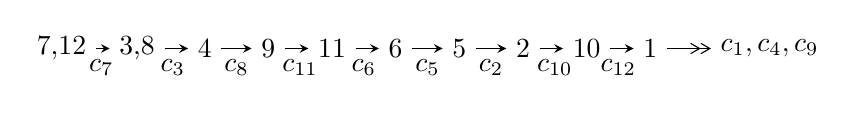
\begin{tikzpicture}[x=23pt, y=7pt]
	% node
	\node (A0) at (-1/8, 0) {7,12};
	\node (A1) at (17/16, 0) {3,8};
	\node (A2) at (17/8, 0) {4};
	\node (A3) at (25/8, 0) {9};
	\node (A4) at (33/8, 0) {11};
	\node (A5) at (41/8, 0) {6};
	\node (A6) at (49/8, 0) {5};
	\node (A7) at (57/8, 0) {2};
	\node (A8) at (65/8, 0) {10};
	\node (A9) at (73/8, 0) {1};
	\node (C1) at (1/2, -1) {$c_{7}$};
	\node (C2) at (13/8, -1) {$c_{3}$};
	\node (C3) at (21/8, -1) {$c_{8}$};
	\node (C4) at (29/8, -1) {$c_{11}$};
	\node (C5) at (37/8, -1) {$c_{6}$};
	\node (C6) at (45/8, -1) {$c_{5}$};
	\node (C7) at (53/8, -1) {$c_{2}$};
	\node (C8) at (61/8, -1) {$c_{10}$};
	\node (C9) at (69/8, -1) {$c_{12}$};
	\node (A10) at (11, 0) {$c_{1},c_{4},c_{9}$};

	% edge
	\draw[->,>=stealth]	
	(A0) edge (A1) (A1) edge (A2) (A2) edge (A3) (A3) edge (A4) (A4) edge (A5) (A5) edge (A6) (A6) edge (A7) (A7) edge (A8) (A8) edge (A9) ;
	\draw[->>,>={angle 60}]	
	(A9) edge (A10);
\end{tikzpicture} \\ 

\end{tabular} \\

\footnotetext{
The image of knot diagram is generated by the software ``\textbf{Draw programme}" developed by Andrew Bartholomew(\url{http://www.layer8.co.uk/maths/draw/index.htm\#Running-draw}), where we modified some parts for our purpose(\url{https://github.com/CATsTAILs/LinksPainter}).
}\phantom \\ \newline 
\centering \textbf{Ideals for irreducible components\footnotemark of $X_{\text{par}}$} 
 
\begin{align*}
I^u_{1}&=\langle 
u^{64}-34 u^{62}+\cdots+b+u,\;- u^{63}+34 u^{61}+\cdots+a-2,\;u^{65}+2 u^{64}+\cdots- u+1\rangle \\
I^u_{2}&=\langle 
u^5-2 u^3- u^2+b+1,\;u^5-3 u^3- u^2+a+2 u+2,\;u^6- u^5-3 u^4+2 u^3+2 u^2+u-1\rangle \\
\\
\end{align*}
\raggedright * 2 irreducible components of $\dim_{\mathbb{C}}=0$, with total 71 representations.\\
\footnotetext{All coefficients of polynomials are rational numbers. But the coefficients are sometimes approximated in decimal forms when there is not enough margin.}
\newpage
\renewcommand{\arraystretch}{1}
\centering \section*{I. $I^u_{1}= \langle u^{64}-34 u^{62}+\cdots+b+u,\;- u^{63}+34 u^{61}+\cdots+a-2,\;u^{65}+2 u^{64}+\cdots- u+1 \rangle$}
\flushleft \textbf{(i) Arc colorings}\\
\begin{tabular}{m{7pt} m{180pt} m{7pt} m{180pt} }
\flushright $a_{7}=$&$\begin{pmatrix}1\\0\end{pmatrix}$ \\
\flushright $a_{12}=$&$\begin{pmatrix}0\\u\end{pmatrix}$ \\
\flushright $a_{3}=$&$\begin{pmatrix}u^{63}-34 u^{61}+\cdots-10 u+2\\- u^{64}+34 u^{62}+\cdots+7 u^2- u\end{pmatrix}$ \\
\flushright $a_{8}=$&$\begin{pmatrix}1\\u^2\end{pmatrix}$ \\
\flushright $a_{4}=$&$\begin{pmatrix}u^{64}+u^{63}+\cdots-12 u+3\\2 u^{64}+2 u^{63}+\cdots-4 u+2\end{pmatrix}$ \\
\flushright $a_{9}=$&$\begin{pmatrix}- u^{11}+6 u^9-12 u^7+8 u^5- u^3+2 u\\- u^{11}+5 u^9-8 u^7+5 u^5-3 u^3+u\end{pmatrix}$ \\
\flushright $a_{11}=$&$\begin{pmatrix}u\\u\end{pmatrix}$ \\
\flushright $a_{6}=$&$\begin{pmatrix}- u^2+1\\- u^2\end{pmatrix}$ \\
\flushright $a_{5}=$&$\begin{pmatrix}u^{20}-11 u^{18}+\cdots-3 u^2+1\\u^{20}-10 u^{18}+40 u^{16}-82 u^{14}+95 u^{12}-72 u^{10}+44 u^8-18 u^6+5 u^4-2 u^2\end{pmatrix}$ \\
\flushright $a_{2}=$&$\begin{pmatrix}u^{64}+u^{63}+\cdots-11 u+3\\u^{64}+u^{63}+\cdots-2 u+1\end{pmatrix}$ \\
\flushright $a_{10}=$&$\begin{pmatrix}- u^3+2 u\\- u^3+u\end{pmatrix}$ \\
\flushright $a_{1}=$&$\begin{pmatrix}- u^7+4 u^5-4 u^3\\- u^7+3 u^5-2 u^3+u\end{pmatrix}$\\&\end{tabular}
\flushleft \textbf{(ii) Obstruction class $= -1$}\\~\\
\flushleft \textbf{(iii) Cusp Shapes $= 8 u^{64}+11 u^{63}+\cdots-22 u-6$}\\~\\
\newpage\renewcommand{\arraystretch}{1}
\flushleft \textbf{(iv) u-Polynomials at the component}\newline \\
\begin{tabular}{m{50pt}|m{274pt}}
Crossings & \hspace{64pt}u-Polynomials at each crossing \\
\hline $$\begin{aligned}c_{1},c_{2},c_{4}\end{aligned}$$&$\begin{aligned}
&u^{65}-7 u^{64}+\cdots-8 u+1
\end{aligned}$\\
\hline $$\begin{aligned}c_{3},c_{8}\end{aligned}$$&$\begin{aligned}
&u^{65}+u^{64}+\cdots+128 u+64
\end{aligned}$\\
\hline $$\begin{aligned}c_{5}\end{aligned}$$&$\begin{aligned}
&u^{65}+2 u^{64}+\cdots-5425 u-1549
\end{aligned}$\\
\hline $$\begin{aligned}c_{6},c_{7},c_{10}\\c_{11}\end{aligned}$$&$\begin{aligned}
&u^{65}-2 u^{64}+\cdots- u-1
\end{aligned}$\\
\hline $$\begin{aligned}c_{9},c_{12}\end{aligned}$$&$\begin{aligned}
&u^{65}-12 u^{64}+\cdots+69 u+73
\end{aligned}$\\
\hline
\end{tabular}\\~\\
\newpage\renewcommand{\arraystretch}{1}
\flushleft \textbf{(v) Riley Polynomials at the component}\newline \\
\begin{tabular}{m{50pt}|m{274pt}}
Crossings & \hspace{64pt}Riley Polynomials at each crossing \\
\hline $$\begin{aligned}c_{1},c_{2},c_{4}\end{aligned}$$&$\begin{aligned}
&y^{65}-63 y^{64}+\cdots+52 y-1
\end{aligned}$\\
\hline $$\begin{aligned}c_{3},c_{8}\end{aligned}$$&$\begin{aligned}
&y^{65}+39 y^{64}+\cdots+12288 y-4096
\end{aligned}$\\
\hline $$\begin{aligned}c_{5}\end{aligned}$$&$\begin{aligned}
&y^{65}-24 y^{64}+\cdots+86536059 y-2399401
\end{aligned}$\\
\hline $$\begin{aligned}c_{6},c_{7},c_{10}\\c_{11}\end{aligned}$$&$\begin{aligned}
&y^{65}-72 y^{64}+\cdots+19 y-1
\end{aligned}$\\
\hline $$\begin{aligned}c_{9},c_{12}\end{aligned}$$&$\begin{aligned}
&y^{65}+36 y^{64}+\cdots+52795 y-5329
\end{aligned}$\\
\hline
\end{tabular}\\~\\
\newpage\flushleft \textbf{(vi) Complex Volumes and Cusp Shapes}
$$\begin{array}{c|c|c}  
\text{Solutions to }I^u_{1}& \I (\text{vol} + \sqrt{-1}CS) & \text{Cusp shape}\\
 \hline 
\begin{aligned}
u &= -0.849078 + 0.151759 I \\
a &= -0.52962 + 2.16096 I \\
b &= -0.290266 + 0.275339 I\end{aligned}
 & -10.18900 + 5.61738 I & -17.6543 - 4.7770 I \\ \hline\begin{aligned}
u &= -0.849078 - 0.151759 I \\
a &= -0.52962 - 2.16096 I \\
b &= -0.290266 - 0.275339 I\end{aligned}
 & -10.18900 - 5.61738 I & -17.6543 + 4.7770 I \\ \hline\begin{aligned}
u &= \phantom{-}0.612809 + 0.581694 I \\
a &= -2.23569 - 1.18411 I \\
b &= \phantom{-}0.116075 - 0.314062 I\end{aligned}
 & -5.66682 - 11.33370 I & -12.3674 + 8.6652 I \\ \hline\begin{aligned}
u &= \phantom{-}0.612809 - 0.581694 I \\
a &= -2.23569 + 1.18411 I \\
b &= \phantom{-}0.116075 + 0.314062 I\end{aligned}
 & -5.66682 + 11.33370 I & -12.3674 - 8.6652 I \\ \hline\begin{aligned}
u &= \phantom{-}0.591829 + 0.558370 I \\
a &= \phantom{-}2.06155 + 1.34040 I \\
b &= -0.355492 + 0.274934 I\end{aligned}
 & \phantom{-}0.33245 - 7.21157 I & -9.35363 + 8.77748 I \\ \hline\begin{aligned}
u &= \phantom{-}0.591829 - 0.558370 I \\
a &= \phantom{-}2.06155 - 1.34040 I \\
b &= -0.355492 - 0.274934 I\end{aligned}
 & \phantom{-}0.33245 + 7.21157 I & -9.35363 - 8.77748 I \\ \hline\begin{aligned}
u &= \phantom{-}0.664359 + 0.450292 I \\
a &= \phantom{-}1.56056 + 0.64097 I \\
b &= -0.296279 - 0.301108 I\end{aligned}
 & -8.31384 - 0.16938 I & -15.5304 + 3.0150 I \\ \hline\begin{aligned}
u &= \phantom{-}0.664359 - 0.450292 I \\
a &= \phantom{-}1.56056 - 0.64097 I \\
b &= -0.296279 + 0.301108 I\end{aligned}
 & -8.31384 + 0.16938 I & -15.5304 - 3.0150 I \\ \hline\begin{aligned}
u &= -0.591992 + 0.536176 I \\
a &= -0.33537 + 1.45599 I \\
b &= -0.242545 + 0.593048 I\end{aligned}
 & -2.33808 + 4.89491 I & -11.39737 - 6.04524 I \\ \hline\begin{aligned}
u &= -0.591992 - 0.536176 I \\
a &= -0.33537 - 1.45599 I \\
b &= -0.242545 - 0.593048 I\end{aligned}
 & -2.33808 - 4.89491 I & -11.39737 + 6.04524 I\\
 \hline 
 \end{array}$$\newpage$$\begin{array}{c|c|c}  
\text{Solutions to }I^u_{1}& \I (\text{vol} + \sqrt{-1}CS) & \text{Cusp shape}\\
 \hline 
\begin{aligned}
u &= -0.494585 + 0.625336 I \\
a &= \phantom{-}0.779520 + 0.719093 I \\
b &= \phantom{-}0.361458 + 0.362562 I\end{aligned}
 & -0.05575 + 2.11893 I & -12.62240 - 3.49033 I \\ \hline\begin{aligned}
u &= -0.494585 - 0.625336 I \\
a &= \phantom{-}0.779520 - 0.719093 I \\
b &= \phantom{-}0.361458 - 0.362562 I\end{aligned}
 & -0.05575 - 2.11893 I & -12.62240 + 3.49033 I \\ \hline\begin{aligned}
u &= \phantom{-}0.774602\phantom{ +0.000000I} \\
a &= \phantom{-}0.765459\phantom{ +0.000000I} \\
b &= -0.650676\phantom{ +0.000000I}\end{aligned}
 & -5.70560\phantom{ +0.000000I} & -17.2280\phantom{ +0.000000I} \\ \hline\begin{aligned}
u &= -0.529854 + 0.558575 I \\
a &= \phantom{-}0.192170 - 0.901830 I \\
b &= \phantom{-}0.116273 - 0.391001 I\end{aligned}
 & \phantom{-}2.87311 + 2.88923 I & -3.42187 - 4.67269 I \\ \hline\begin{aligned}
u &= -0.529854 - 0.558575 I \\
a &= \phantom{-}0.192170 + 0.901830 I \\
b &= \phantom{-}0.116273 + 0.391001 I\end{aligned}
 & \phantom{-}2.87311 - 2.88923 I & -3.42187 + 4.67269 I \\ \hline\begin{aligned}
u &= \phantom{-}0.573094 + 0.509493 I \\
a &= -1.56952 - 1.35973 I \\
b &= \phantom{-}0.564918 + 0.034458 I\end{aligned}
 & -0.92967 - 2.31652 I & -12.22093 + 3.86577 I \\ \hline\begin{aligned}
u &= \phantom{-}0.573094 - 0.509493 I \\
a &= -1.56952 + 1.35973 I \\
b &= \phantom{-}0.564918 - 0.034458 I\end{aligned}
 & -0.92967 + 2.31652 I & -12.22093 - 3.86577 I \\ \hline\begin{aligned}
u &= -0.761928 + 0.069316 I \\
a &= \phantom{-}0.34486 - 2.57712 I \\
b &= \phantom{-}0.144740 - 0.449027 I\end{aligned}
 & -3.63927 + 2.31291 I & -16.5119 - 4.5602 I \\ \hline\begin{aligned}
u &= -0.761928 - 0.069316 I \\
a &= \phantom{-}0.34486 + 2.57712 I \\
b &= \phantom{-}0.144740 + 0.449027 I\end{aligned}
 & -3.63927 - 2.31291 I & -16.5119 + 4.5602 I \\ \hline\begin{aligned}
u &= -0.444280 + 0.563851 I \\
a &= -0.979188 + 0.166649 I \\
b &= -0.439103 + 0.089481 I\end{aligned}
 & \phantom{-}3.12509 + 0.97162 I & -2.56463 - 3.01871 I\\
 \hline 
 \end{array}$$\newpage$$\begin{array}{c|c|c}  
\text{Solutions to }I^u_{1}& \I (\text{vol} + \sqrt{-1}CS) & \text{Cusp shape}\\
 \hline 
\begin{aligned}
u &= -0.444280 - 0.563851 I \\
a &= -0.979188 - 0.166649 I \\
b &= -0.439103 - 0.089481 I\end{aligned}
 & \phantom{-}3.12509 - 0.97162 I & -2.56463 + 3.01871 I \\ \hline\begin{aligned}
u &= \phantom{-}0.345558 + 0.625959 I \\
a &= \phantom{-}0.597480 + 0.424044 I \\
b &= \phantom{-}0.26840 + 1.44188 I\end{aligned}
 & -4.88166 + 7.23122 I & -10.46990 - 2.83323 I \\ \hline\begin{aligned}
u &= \phantom{-}0.345558 - 0.625959 I \\
a &= \phantom{-}0.597480 - 0.424044 I \\
b &= \phantom{-}0.26840 - 1.44188 I\end{aligned}
 & -4.88166 - 7.23122 I & -10.46990 + 2.83323 I \\ \hline\begin{aligned}
u &= \phantom{-}0.360635 + 0.581410 I \\
a &= -0.519658 + 0.056262 I \\
b &= -0.363851 - 1.310020 I\end{aligned}
 & \phantom{-}1.00659 + 3.30244 I & -7.13975 - 2.59787 I \\ \hline\begin{aligned}
u &= \phantom{-}0.360635 - 0.581410 I \\
a &= -0.519658 - 0.056262 I \\
b &= -0.363851 + 1.310020 I\end{aligned}
 & \phantom{-}1.00659 - 3.30244 I & -7.13975 + 2.59787 I \\ \hline\begin{aligned}
u &= -0.347239 + 0.544294 I \\
a &= \phantom{-}1.54475 - 0.29359 I \\
b &= \phantom{-}0.667710 - 0.250220 I\end{aligned}
 & -1.63173 - 1.15310 I & -8.96204 - 0.62633 I \\ \hline\begin{aligned}
u &= -0.347239 - 0.544294 I \\
a &= \phantom{-}1.54475 + 0.29359 I \\
b &= \phantom{-}0.667710 + 0.250220 I\end{aligned}
 & -1.63173 + 1.15310 I & -8.96204 + 0.62633 I \\ \hline\begin{aligned}
u &= \phantom{-}0.397848 + 0.479108 I \\
a &= -0.152635 - 0.791660 I \\
b &= \phantom{-}0.493556 + 0.869041 I\end{aligned}
 & -0.383917 - 1.172590 I & -10.77474 + 3.53972 I \\ \hline\begin{aligned}
u &= \phantom{-}0.397848 - 0.479108 I \\
a &= -0.152635 + 0.791660 I \\
b &= \phantom{-}0.493556 - 0.869041 I\end{aligned}
 & -0.383917 + 1.172590 I & -10.77474 - 3.53972 I \\ \hline\begin{aligned}
u &= -1.40989 + 0.11554 I \\
a &= -0.085739 - 0.727029 I \\
b &= -0.963524 - 0.159703 I\end{aligned}
 & -10.37080 - 4.63328 I & \phantom{-0.000000 } 0\\
 \hline 
 \end{array}$$\newpage$$\begin{array}{c|c|c}  
\text{Solutions to }I^u_{1}& \I (\text{vol} + \sqrt{-1}CS) & \text{Cusp shape}\\
 \hline 
\begin{aligned}
u &= -1.40989 - 0.11554 I \\
a &= -0.085739 + 0.727029 I \\
b &= -0.963524 + 0.159703 I\end{aligned}
 & -10.37080 + 4.63328 I & \phantom{-0.000000 } 0 \\ \hline\begin{aligned}
u &= \phantom{-}0.163296 + 0.550521 I \\
a &= \phantom{-}0.765667 - 0.368871 I \\
b &= \phantom{-}0.216553 - 1.080350 I\end{aligned}
 & -6.83780 - 3.22697 I & -11.27004 + 3.16299 I \\ \hline\begin{aligned}
u &= \phantom{-}0.163296 - 0.550521 I \\
a &= \phantom{-}0.765667 + 0.368871 I \\
b &= \phantom{-}0.216553 + 1.080350 I\end{aligned}
 & -6.83780 + 3.22697 I & -11.27004 - 3.16299 I \\ \hline\begin{aligned}
u &= \phantom{-}0.544767\phantom{ +0.000000I} \\
a &= -0.440631\phantom{ +0.000000I} \\
b &= \phantom{-}0.243537\phantom{ +0.000000I}\end{aligned}
 & -0.894856\phantom{ +0.000000I} & -10.6250\phantom{ +0.000000I} \\ \hline\begin{aligned}
u &= -1.46159 + 0.10569 I \\
a &= \phantom{-}0.181952 + 0.962693 I \\
b &= \phantom{-}1.16904 + 1.01325 I\end{aligned}
 & -4.78459 - 1.02708 I & \phantom{-0.000000 } 0 \\ \hline\begin{aligned}
u &= -1.46159 - 0.10569 I \\
a &= \phantom{-}0.181952 - 0.962693 I \\
b &= \phantom{-}1.16904 - 1.01325 I\end{aligned}
 & -4.78459 + 1.02708 I & \phantom{-0.000000 } 0 \\ \hline\begin{aligned}
u &= \phantom{-}1.49086 + 0.09279 I \\
a &= -0.707400 - 0.841672 I \\
b &= -2.22656 - 1.64975 I\end{aligned}
 & -7.55431 - 0.79217 I & \phantom{-0.000000 } 0 \\ \hline\begin{aligned}
u &= \phantom{-}1.49086 - 0.09279 I \\
a &= -0.707400 + 0.841672 I \\
b &= -2.22656 + 1.64975 I\end{aligned}
 & -7.55431 + 0.79217 I & \phantom{-0.000000 } 0 \\ \hline\begin{aligned}
u &= \phantom{-}1.50040 + 0.14327 I \\
a &= \phantom{-}0.388062 + 0.569649 I \\
b &= \phantom{-}1.27751 + 0.96561 I\end{aligned}
 & -3.25528 - 3.41758 I & \phantom{-0.000000 } 0 \\ \hline\begin{aligned}
u &= \phantom{-}1.50040 - 0.14327 I \\
a &= \phantom{-}0.388062 - 0.569649 I \\
b &= \phantom{-}1.27751 - 0.96561 I\end{aligned}
 & -3.25528 + 3.41758 I & \phantom{-0.000000 } 0\\
 \hline 
 \end{array}$$\newpage$$\begin{array}{c|c|c}  
\text{Solutions to }I^u_{1}& \I (\text{vol} + \sqrt{-1}CS) & \text{Cusp shape}\\
 \hline 
\begin{aligned}
u &= -1.51289 + 0.11377 I \\
a &= \phantom{-}0.01624 - 1.55519 I \\
b &= -0.88043 - 2.69896 I\end{aligned}
 & -6.78772 + 3.13550 I & \phantom{-0.000000 } 0 \\ \hline\begin{aligned}
u &= -1.51289 - 0.11377 I \\
a &= \phantom{-}0.01624 + 1.55519 I \\
b &= -0.88043 + 2.69896 I\end{aligned}
 & -6.78772 - 3.13550 I & \phantom{-0.000000 } 0 \\ \hline\begin{aligned}
u &= \phantom{-}1.50743 + 0.18519 I \\
a &= -0.660901 - 0.183350 I \\
b &= -1.47488 + 0.16745 I\end{aligned}
 & -6.61480 - 5.02407 I & \phantom{-0.000000 } 0 \\ \hline\begin{aligned}
u &= \phantom{-}1.50743 - 0.18519 I \\
a &= -0.660901 + 0.183350 I \\
b &= -1.47488 - 0.16745 I\end{aligned}
 & -6.61480 + 5.02407 I & \phantom{-0.000000 } 0 \\ \hline\begin{aligned}
u &= \phantom{-}1.53689 + 0.16083 I \\
a &= \phantom{-}0.347709 - 0.503738 I \\
b &= \phantom{-}0.381409 - 1.252670 I\end{aligned}
 & -3.99527 - 5.46572 I & \phantom{-0.000000 } 0 \\ \hline\begin{aligned}
u &= \phantom{-}1.53689 - 0.16083 I \\
a &= \phantom{-}0.347709 + 0.503738 I \\
b &= \phantom{-}0.381409 + 1.252670 I\end{aligned}
 & -3.99527 + 5.46572 I & \phantom{-0.000000 } 0 \\ \hline\begin{aligned}
u &= -1.55420\phantom{ +0.000000I} \\
a &= \phantom{-}0.565237\phantom{ +0.000000I} \\
b &= \phantom{-}0.840718\phantom{ +0.000000I}\end{aligned}
 & -8.08338\phantom{ +0.000000I} & \phantom{-0.000000 } 0 \\ \hline\begin{aligned}
u &= -1.55791 + 0.14949 I \\
a &= \phantom{-}1.11591 - 2.21291 I \\
b &= \phantom{-}1.77120 - 4.71029 I\end{aligned}
 & -8.07881 + 4.70967 I & \phantom{-0.000000 } 0 \\ \hline\begin{aligned}
u &= -1.55791 - 0.14949 I \\
a &= \phantom{-}1.11591 + 2.21291 I \\
b &= \phantom{-}1.77120 + 4.71029 I\end{aligned}
 & -8.07881 - 4.70967 I & \phantom{-0.000000 } 0 \\ \hline\begin{aligned}
u &= -1.56117 + 0.16671 I \\
a &= -1.34382 + 2.19591 I \\
b &= -2.54714 + 4.80810 I\end{aligned}
 & -6.86256 + 9.85745 I & \phantom{-0.000000 } 0\\
 \hline 
 \end{array}$$\newpage$$\begin{array}{c|c|c}  
\text{Solutions to }I^u_{1}& \I (\text{vol} + \sqrt{-1}CS) & \text{Cusp shape}\\
 \hline 
\begin{aligned}
u &= -1.56117 - 0.16671 I \\
a &= -1.34382 - 2.19591 I \\
b &= -2.54714 - 4.80810 I\end{aligned}
 & -6.86256 - 9.85745 I & \phantom{-0.000000 } 0 \\ \hline\begin{aligned}
u &= \phantom{-}1.56229 + 0.15874 I \\
a &= -0.629847 + 0.881225 I \\
b &= -0.75213 + 2.10739 I\end{aligned}
 & -9.55235 - 7.42892 I & \phantom{-0.000000 } 0 \\ \hline\begin{aligned}
u &= \phantom{-}1.56229 - 0.15874 I \\
a &= -0.629847 - 0.881225 I \\
b &= -0.75213 - 2.10739 I\end{aligned}
 & -9.55235 + 7.42892 I & \phantom{-0.000000 } 0 \\ \hline\begin{aligned}
u &= -1.56850 + 0.17675 I \\
a &= \phantom{-}1.36052 - 2.11880 I \\
b &= \phantom{-}2.79633 - 4.55461 I\end{aligned}
 & -12.9536 + 14.1196 I & \phantom{-0.000000 } 0 \\ \hline\begin{aligned}
u &= -1.56850 - 0.17675 I \\
a &= \phantom{-}1.36052 + 2.11880 I \\
b &= \phantom{-}2.79633 + 4.55461 I\end{aligned}
 & -12.9536 - 14.1196 I & \phantom{-0.000000 } 0 \\ \hline\begin{aligned}
u &= -1.58211 + 0.12862 I \\
a &= -1.21036 + 1.81529 I \\
b &= -2.00477 + 3.54223 I\end{aligned}
 & -15.8923 + 2.2931 I & \phantom{-0.000000 } 0 \\ \hline\begin{aligned}
u &= -1.58211 - 0.12862 I \\
a &= -1.21036 - 1.81529 I \\
b &= -2.00477 - 3.54223 I\end{aligned}
 & -15.8923 - 2.2931 I & \phantom{-0.000000 } 0 \\ \hline\begin{aligned}
u &= \phantom{-}1.59363 + 0.01214 I \\
a &= -0.09196 - 2.88914 I \\
b &= -0.32386 - 6.15827 I\end{aligned}
 & -11.62670 - 2.56811 I & \phantom{-0.000000 } 0 \\ \hline\begin{aligned}
u &= \phantom{-}1.59363 - 0.01214 I \\
a &= -0.09196 + 2.88914 I \\
b &= -0.32386 + 6.15827 I\end{aligned}
 & -11.62670 + 2.56811 I & \phantom{-0.000000 } 0 \\ \hline\begin{aligned}
u &= -1.59618\phantom{ +0.000000I} \\
a &= -1.28300\phantom{ +0.000000I} \\
b &= -2.03922\phantom{ +0.000000I}\end{aligned}
 & -13.7436\phantom{ +0.000000I} & \phantom{-0.000000 } 0\\
 \hline 
 \end{array}$$\newpage$$\begin{array}{c|c|c}  
\text{Solutions to }I^u_{1}& \I (\text{vol} + \sqrt{-1}CS) & \text{Cusp shape}\\
 \hline 
\begin{aligned}
u &= \phantom{-}0.220404 + 0.332017 I \\
a &= -0.864656 - 0.515239 I \\
b &= -0.008971 + 0.638980 I\end{aligned}
 & -0.505584 - 0.990498 I & -8.02418 + 6.33094 I \\ \hline\begin{aligned}
u &= \phantom{-}0.220404 - 0.332017 I \\
a &= -0.864656 + 0.515239 I \\
b &= -0.008971 - 0.638980 I\end{aligned}
 & -0.505584 + 0.990498 I & -8.02418 - 6.33094 I \\ \hline\begin{aligned}
u &= \phantom{-}1.61071 + 0.02844 I \\
a &= \phantom{-}0.00288 + 2.74367 I \\
b &= \phantom{-}0.26375 + 5.67324 I\end{aligned}
 & -18.5211 - 6.1970 I & \phantom{-0.000000 } 0 \\ \hline\begin{aligned}
u &= \phantom{-}1.61071 - 0.02844 I \\
a &= \phantom{-}0.00288 - 2.74367 I \\
b &= \phantom{-}0.26375 - 5.67324 I\end{aligned}
 & -18.5211 + 6.1970 I & \phantom{-0.000000 } 0 \\ \hline\begin{aligned}
u &= -0.287026\phantom{ +0.000000I} \\
a &= \phantom{-}3.70600\phantom{ +0.000000I} \\
b &= \phantom{-}0.727372\phantom{ +0.000000I}\end{aligned}
 & -2.04090\phantom{ +0.000000I} & \phantom{-}0.885750\phantom{ +0.000000I}\\
 \hline 
 \end{array}$$\newpage\newpage\renewcommand{\arraystretch}{1}
\centering \section*{II. $I^u_{2}= \langle u^5-2 u^3- u^2+b+1,\;u^5-3 u^3- u^2+a+2 u+2,\;u^6- u^5-3 u^4+2 u^3+2 u^2+u-1 \rangle$}
\flushleft \textbf{(i) Arc colorings}\\
\begin{tabular}{m{7pt} m{180pt} m{7pt} m{180pt} }
\flushright $a_{7}=$&$\begin{pmatrix}1\\0\end{pmatrix}$ \\
\flushright $a_{12}=$&$\begin{pmatrix}0\\u\end{pmatrix}$ \\
\flushright $a_{3}=$&$\begin{pmatrix}- u^5+3 u^3+u^2-2 u-2\\- u^5+2 u^3+u^2-1\end{pmatrix}$ \\
\flushright $a_{8}=$&$\begin{pmatrix}1\\u^2\end{pmatrix}$ \\
\flushright $a_{4}=$&$\begin{pmatrix}- u^5+3 u^3+u^2-2 u-2\\- u^5+2 u^3+u^2-1\end{pmatrix}$ \\
\flushright $a_{9}=$&$\begin{pmatrix}1\\u^2\end{pmatrix}$ \\
\flushright $a_{11}=$&$\begin{pmatrix}u\\u\end{pmatrix}$ \\
\flushright $a_{6}=$&$\begin{pmatrix}- u^2+1\\- u^2\end{pmatrix}$ \\
\flushright $a_{5}=$&$\begin{pmatrix}u^4-3 u^2+1\\u^5+u^4-2 u^3-3 u^2- u+1\end{pmatrix}$ \\
\flushright $a_{2}=$&$\begin{pmatrix}- u^5- u^4+3 u^3+4 u^2-2 u-3\\-2 u^5- u^4+4 u^3+4 u^2+u-2\end{pmatrix}$ \\
\flushright $a_{10}=$&$\begin{pmatrix}- u^3+2 u\\- u^3+u\end{pmatrix}$ \\
\flushright $a_{1}=$&$\begin{pmatrix}- u^4+3 u^2-1\\- u^5- u^4+2 u^3+3 u^2+u-1\end{pmatrix}$\\&\end{tabular}
\flushleft \textbf{(ii) Obstruction class $= 1$}\\~\\
\flushleft \textbf{(iii) Cusp Shapes $= -3 u^5+u^4+14 u^3- u^2-14 u-18$}\\~\\
\newpage\renewcommand{\arraystretch}{1}
\flushleft \textbf{(iv) u-Polynomials at the component}\newline \\
\begin{tabular}{m{50pt}|m{274pt}}
Crossings & \hspace{64pt}u-Polynomials at each crossing \\
\hline $$\begin{aligned}c_{1},c_{2}\end{aligned}$$&$\begin{aligned}
&(u-1)^6
\end{aligned}$\\
\hline $$\begin{aligned}c_{3},c_{8}\end{aligned}$$&$\begin{aligned}
&u^6
\end{aligned}$\\
\hline $$\begin{aligned}c_{4}\end{aligned}$$&$\begin{aligned}
&(u+1)^6
\end{aligned}$\\
\hline $$\begin{aligned}c_{5},c_{9}\end{aligned}$$&$\begin{aligned}
&u^6+u^5+3 u^4+2 u^3+2 u^2+u-1
\end{aligned}$\\
\hline $$\begin{aligned}c_{6},c_{7}\end{aligned}$$&$\begin{aligned}
&u^6- u^5-3 u^4+2 u^3+2 u^2+u-1
\end{aligned}$\\
\hline $$\begin{aligned}c_{10},c_{11}\end{aligned}$$&$\begin{aligned}
&u^6+u^5-3 u^4-2 u^3+2 u^2- u-1
\end{aligned}$\\
\hline $$\begin{aligned}c_{12}\end{aligned}$$&$\begin{aligned}
&u^6- u^5+3 u^4-2 u^3+2 u^2- u-1
\end{aligned}$\\
\hline
\end{tabular}\\~\\
\newpage\renewcommand{\arraystretch}{1}
\flushleft \textbf{(v) Riley Polynomials at the component}\newline \\
\begin{tabular}{m{50pt}|m{274pt}}
Crossings & \hspace{64pt}Riley Polynomials at each crossing \\
\hline $$\begin{aligned}c_{1},c_{2},c_{4}\end{aligned}$$&$\begin{aligned}
&(y-1)^6
\end{aligned}$\\
\hline $$\begin{aligned}c_{3},c_{8}\end{aligned}$$&$\begin{aligned}
&y^6
\end{aligned}$\\
\hline $$\begin{aligned}c_{5},c_{9},c_{12}\end{aligned}$$&$\begin{aligned}
&y^6+5 y^5+9 y^4+4 y^3-6 y^2-5 y+1
\end{aligned}$\\
\hline $$\begin{aligned}c_{6},c_{7},c_{10}\\c_{11}\end{aligned}$$&$\begin{aligned}
&y^6-7 y^5+17 y^4-16 y^3+6 y^2-5 y+1
\end{aligned}$\\
\hline
\end{tabular}\\~\\
\newpage\flushleft \textbf{(vi) Complex Volumes and Cusp Shapes}
$$\begin{array}{c|c|c}  
\text{Solutions to }I^u_{2}& \I (\text{vol} + \sqrt{-1}CS) & \text{Cusp shape}\\
 \hline 
\begin{aligned}
u &= -0.493180 + 0.575288 I \\
a &= -0.089969 - 0.799962 I \\
b &= -0.446039 + 0.121233 I\end{aligned}
 & \phantom{-}1.31531 + 1.97241 I & -6.43930 - 3.48596 I \\ \hline\begin{aligned}
u &= -0.493180 - 0.575288 I \\
a &= -0.089969 + 0.799962 I \\
b &= -0.446039 - 0.121233 I\end{aligned}
 & \phantom{-}1.31531 - 1.97241 I & -6.43930 + 3.48596 I \\ \hline\begin{aligned}
u &= \phantom{-}0.483672\phantom{ +0.000000I} \\
a &= -2.42043\phantom{ +0.000000I} \\
b &= -0.566232\phantom{ +0.000000I}\end{aligned}
 & -2.38379\phantom{ +0.000000I} & -23.4460\phantom{ +0.000000I} \\ \hline\begin{aligned}
u &= \phantom{-}1.52087 + 0.16310 I \\
a &= \phantom{-}0.227586 - 0.710576 I \\
b &= \phantom{-}0.87287 - 1.51178 I\end{aligned}
 & -5.34051 - 4.59213 I & -10.66600 + 2.48468 I \\ \hline\begin{aligned}
u &= \phantom{-}1.52087 - 0.16310 I \\
a &= \phantom{-}0.227586 + 0.710576 I \\
b &= \phantom{-}0.87287 + 1.51178 I\end{aligned}
 & -5.34051 + 4.59213 I & -10.66600 - 2.48468 I \\ \hline\begin{aligned}
u &= -1.53904\phantom{ +0.000000I} \\
a &= \phantom{-}1.14519\phantom{ +0.000000I} \\
b &= \phantom{-}2.71257\phantom{ +0.000000I}\end{aligned}
 & -9.30502\phantom{ +0.000000I} & -18.3430\phantom{ +0.000000I}\\
 \hline 
 \end{array}$$\newpage
\newpage\renewcommand{\arraystretch}{1}
\centering \section*{ III. u-Polynomials}
\begin{tabular}{m{50pt}|m{274pt}}
Crossings & \hspace{64pt}u-Polynomials at each crossing \\
\hline $$\begin{aligned}c_{1},c_{2}\end{aligned}$$&$\begin{aligned}
&((u-1)^6)(u^{65}-7 u^{64}+\cdots-8 u+1)
\end{aligned}$\\
\hline $$\begin{aligned}c_{3},c_{8}\end{aligned}$$&$\begin{aligned}
&u^6(u^{65}+u^{64}+\cdots+128 u+64)
\end{aligned}$\\
\hline $$\begin{aligned}c_{4}\end{aligned}$$&$\begin{aligned}
&((u+1)^6)(u^{65}-7 u^{64}+\cdots-8 u+1)
\end{aligned}$\\
\hline $$\begin{aligned}c_{5}\end{aligned}$$&$\begin{aligned}
&(u^6+u^5+3 u^4+2 u^3+2 u^2+u-1)(u^{65}+2 u^{64}+\cdots-5425 u-1549)
\end{aligned}$\\
\hline $$\begin{aligned}c_{6},c_{7}\end{aligned}$$&$\begin{aligned}
&(u^6- u^5-3 u^4+2 u^3+2 u^2+u-1)(u^{65}-2 u^{64}+\cdots- u-1)
\end{aligned}$\\
\hline $$\begin{aligned}c_{9}\end{aligned}$$&$\begin{aligned}
&(u^6+u^5+3 u^4+2 u^3+2 u^2+u-1)(u^{65}-12 u^{64}+\cdots+69 u+73)
\end{aligned}$\\
\hline $$\begin{aligned}c_{10},c_{11}\end{aligned}$$&$\begin{aligned}
&(u^6+u^5-3 u^4-2 u^3+2 u^2- u-1)(u^{65}-2 u^{64}+\cdots- u-1)
\end{aligned}$\\
\hline $$\begin{aligned}c_{12}\end{aligned}$$&$\begin{aligned}
&(u^6- u^5+3 u^4-2 u^3+2 u^2- u-1)(u^{65}-12 u^{64}+\cdots+69 u+73)
\end{aligned}$\\
\hline
\end{tabular}\newpage\renewcommand{\arraystretch}{1}
\centering \section*{ IV. Riley Polynomials}
\begin{tabular}{m{50pt}|m{274pt}}
Crossings & \hspace{64pt}Riley Polynomials at each crossing \\
\hline $$\begin{aligned}c_{1},c_{2},c_{4}\end{aligned}$$&$\begin{aligned}
&((y-1)^6)(y^{65}-63 y^{64}+\cdots+52 y-1)
\end{aligned}$\\
\hline $$\begin{aligned}c_{3},c_{8}\end{aligned}$$&$\begin{aligned}
&y^6(y^{65}+39 y^{64}+\cdots+12288 y-4096)
\end{aligned}$\\
\hline $$\begin{aligned}c_{5}\end{aligned}$$&$\begin{aligned}
&(y^6+5 y^5+9 y^4+4 y^3-6 y^2-5 y+1)\\
&\cdot(y^{65}-24 y^{64}+\cdots+86536059 y-2399401)
\end{aligned}$\\
\hline $$\begin{aligned}c_{6},c_{7},c_{10}\\c_{11}\end{aligned}$$&$\begin{aligned}
&(y^6-7 y^5+\cdots-5 y+1)(y^{65}-72 y^{64}+\cdots+19 y-1)
\end{aligned}$\\
\hline $$\begin{aligned}c_{9},c_{12}\end{aligned}$$&$\begin{aligned}
&(y^6+5 y^5+9 y^4+4 y^3-6 y^2-5 y+1)\\
&\cdot(y^{65}+36 y^{64}+\cdots+52795 y-5329)
\end{aligned}$\\
\hline
\end{tabular}
\vskip 2pc
\end{document}